\section{Introducción}

\subsection{Historia}

% Historia de los sistemas de visión artificial.Inspiración en la visión humana. Elementos que constituyen un sistema de visión artificial.

\begin{figure}[h]
  \centerfloat
  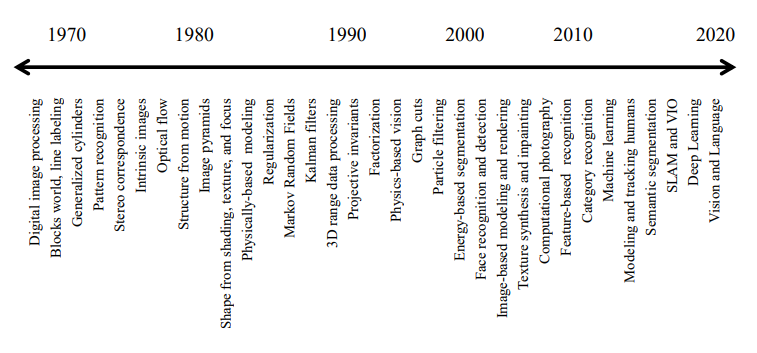
\includegraphics[width=0.75\textwidth]{img/history.png}
  \caption{Eventos destacables en la historia de la visión artificial.}
\end{figure}

La visión artificial comienza a plantearse en los años 60, después de que Larry Roberts propusiera la extracción de información geométrica a partir de fotografías 2D.
Sus primeras aproximaciones trataban tareas específicas como la detección de bordes o la identificación de patrones, basándose en técnicas matemáticas rigurosas.
Durante los 80 siguió el énfasis en explorar las distintas técnicas matemáticas y se plantean las primeras ideas de CNN. Entre algunas de las aplicaciones se comienzan a usar las pirámides para la mezcla y para el manejo de imágenes multi-escala.
En los 90 surge un mayor esfuerzo en resolver problemas de movimiento. También aumenta el número de aplicaciones relacionadas con gráficos, como la modelización y representación de imágenes 3D.

\vspace{\baselineskip}

A comienzos del siglo XXI cambia la aproximación clásica de crear buenos modelos matemáticos con características cuidadosamente extraídas por un enfoque en el aprendizaje de características a partir de los datos bajo la asunción de que múltiples conceptos son compartidos. Entre algunas de las aplicaciones está el primer framework de detección de caras a tiempo real (Viola-Jones) y el inicio de la experimentación con coches autónomos.

\vspace{\baselineskip}

Durante la década pasada sigue la tendencia de usar grandes bases de datos para desarrollar algoritmos de aprendizaje, y en 2012 comienza la expansión del aprendizaje profundo cuando la arquitectura AlexNet gana la competición ImageNet. A partir de entonces se diversifica el uso de la visión artificial en múltiples campos diferentes, la mayoría basándose en el potencial de estas nuevas técnicas.

% 60s: La visión artificial comienza a plantearse en los años 60, después de que Larry Roberts propusiera la extracción de información geométrica a partir de fotografías 2D.

% 70s: Los primeros intentos pretendían la detección de bordes y la identificación de patrones.

% 80s: Se comienza a aplicar un mayor énfasis en técnicas matemáticas y se plantean primeras ideas de CNN. Se comienzan a usar las pirámides de imágenes para la mezcla de imágenes y para el manejo de imágenes multi-escala.

% 90s: Múltiples esfuerzos en resolver problemas de movimiento y en la modelización y representación de imágenes 3D.

% 00s: Mayor influencia de los sistemas de aprendizaje dirigidos por datos. Surge una tendencia a aplicar técnicas basadas en características para la clasificación de objetos. Se introduce el primer framework de detección de caras a tiempo real (Viola-Jones). Google comienza su experimentación con coches autónomos

% Cambia la aproximación clásica de crear buenos modelos matemáticos con características cuidadosamente extraídas por un enfoque en el aprendizaje de características a partir de los datos bajo la asunción de que múltiples conceptos comparten características.

% 10s: Sigue la tendencia de usar grandes bases de datos para desarrollar algoritmos de aprendizaje. Se expande el uso de de reconocimiento de caras (redes sociales, seguridad\dots).


\begin{figure}[H]
    \centerfloat
    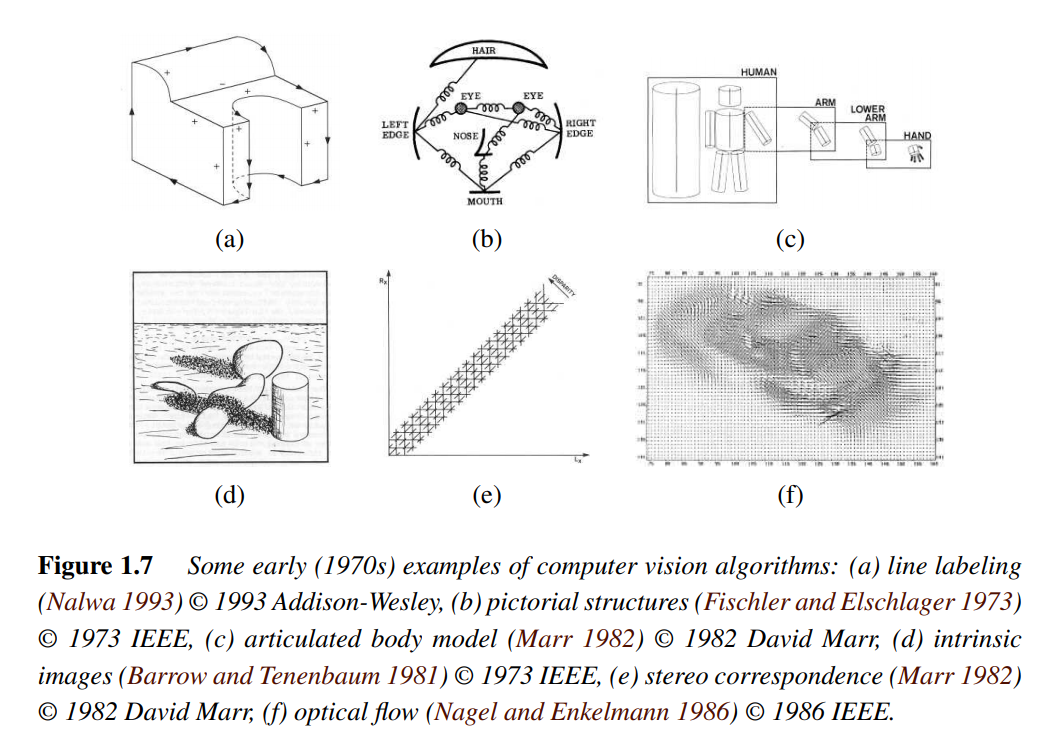
\includegraphics[width=0.75\textwidth]{img/70s.png}
\end{figure}

\begin{figure}[H]
    \centerfloat
    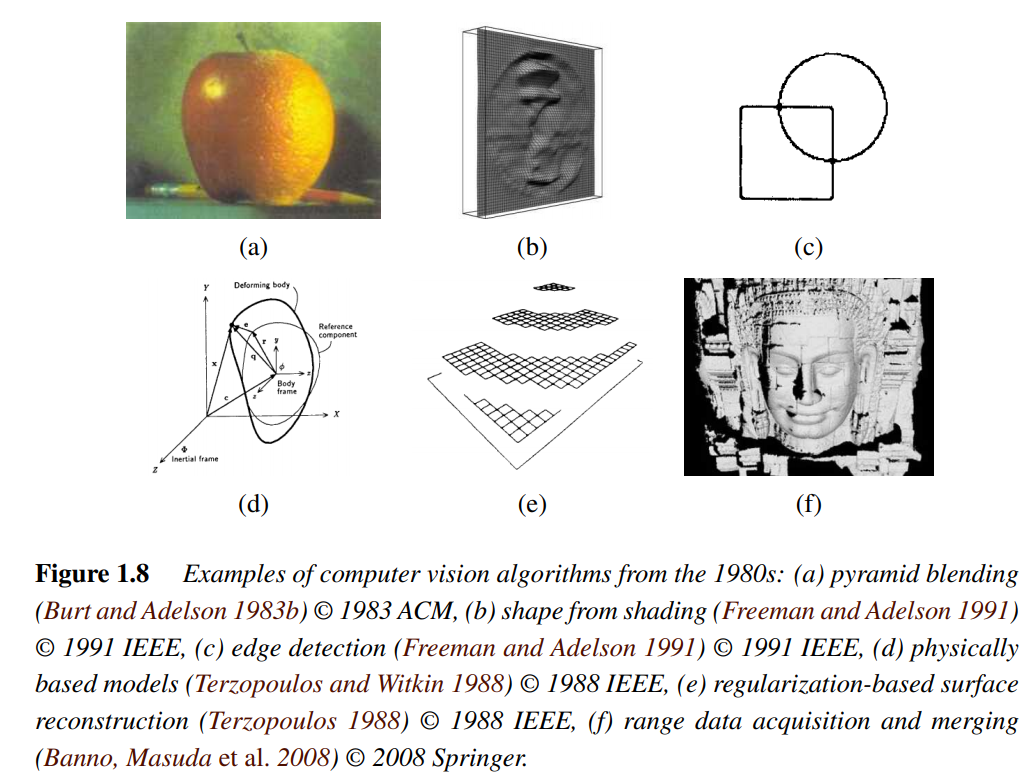
\includegraphics[width=0.75\textwidth]{img/80s.png}
\end{figure}

\begin{figure}[H]
    \centerfloat
    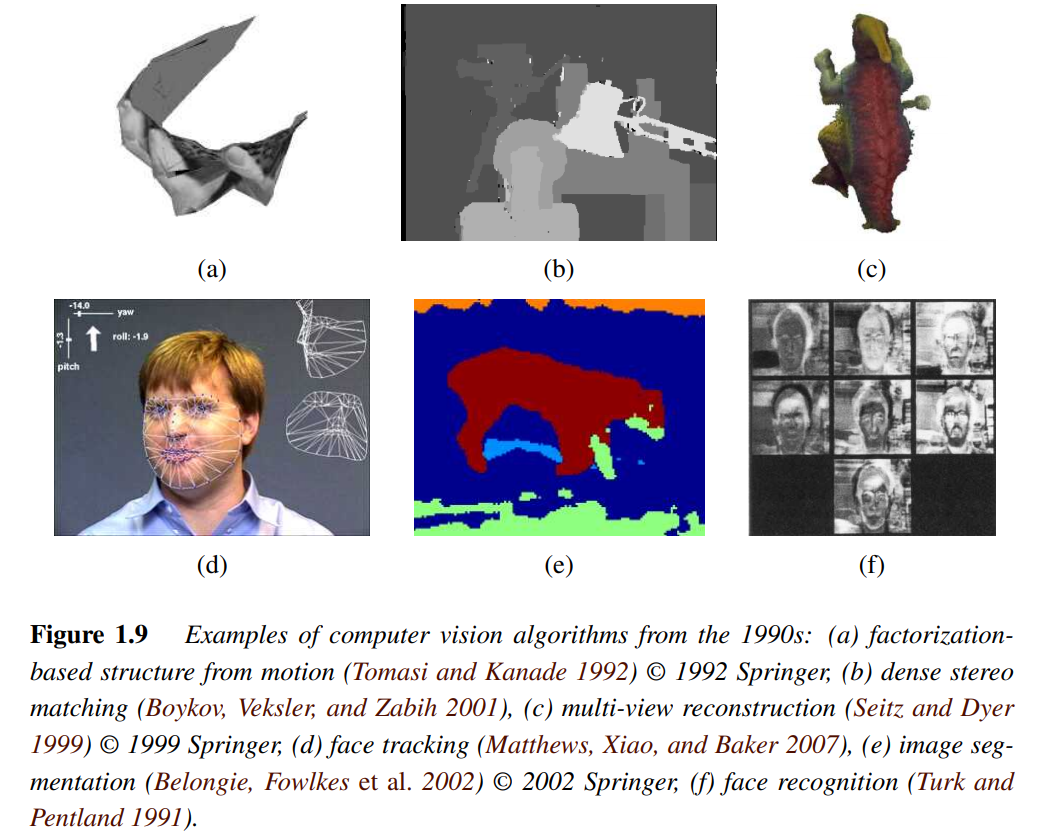
\includegraphics[width=0.75\textwidth]{img/90s.png}
\end{figure}

\begin{figure}[H]
    \centerfloat
    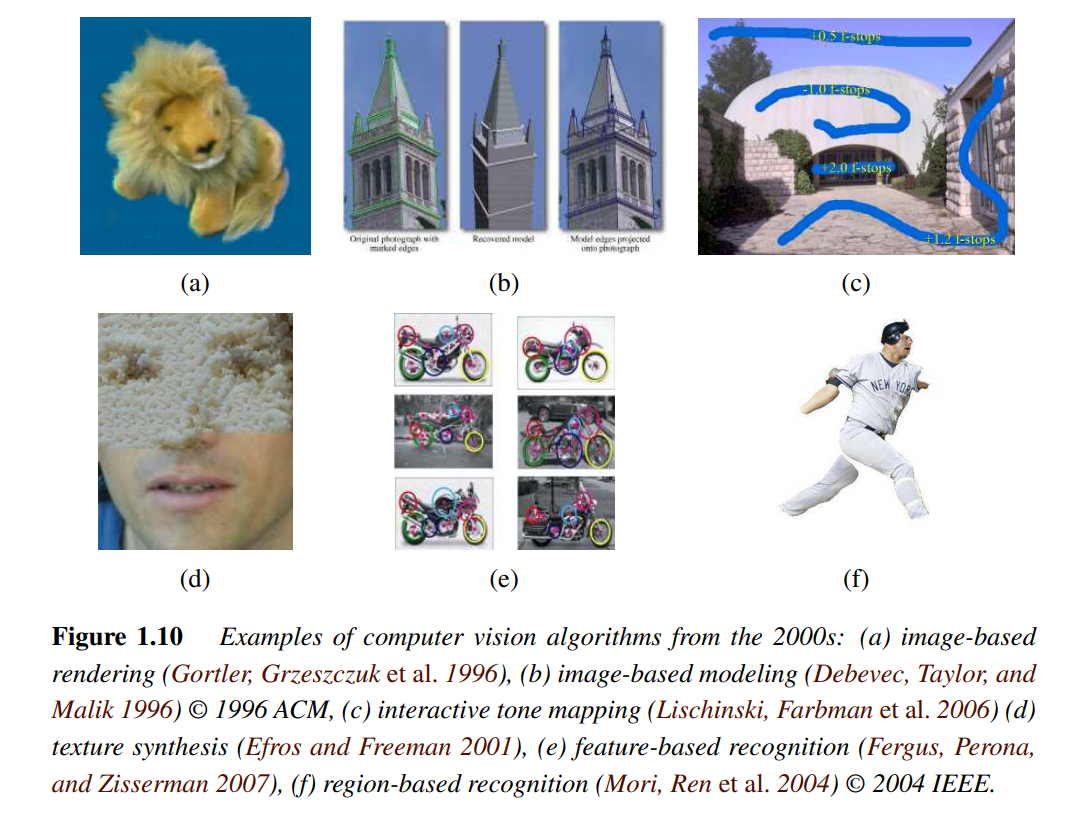
\includegraphics[width=0.75\textwidth]{img/00s.png}
\end{figure}

\begin{figure}[H]
    \centerfloat
    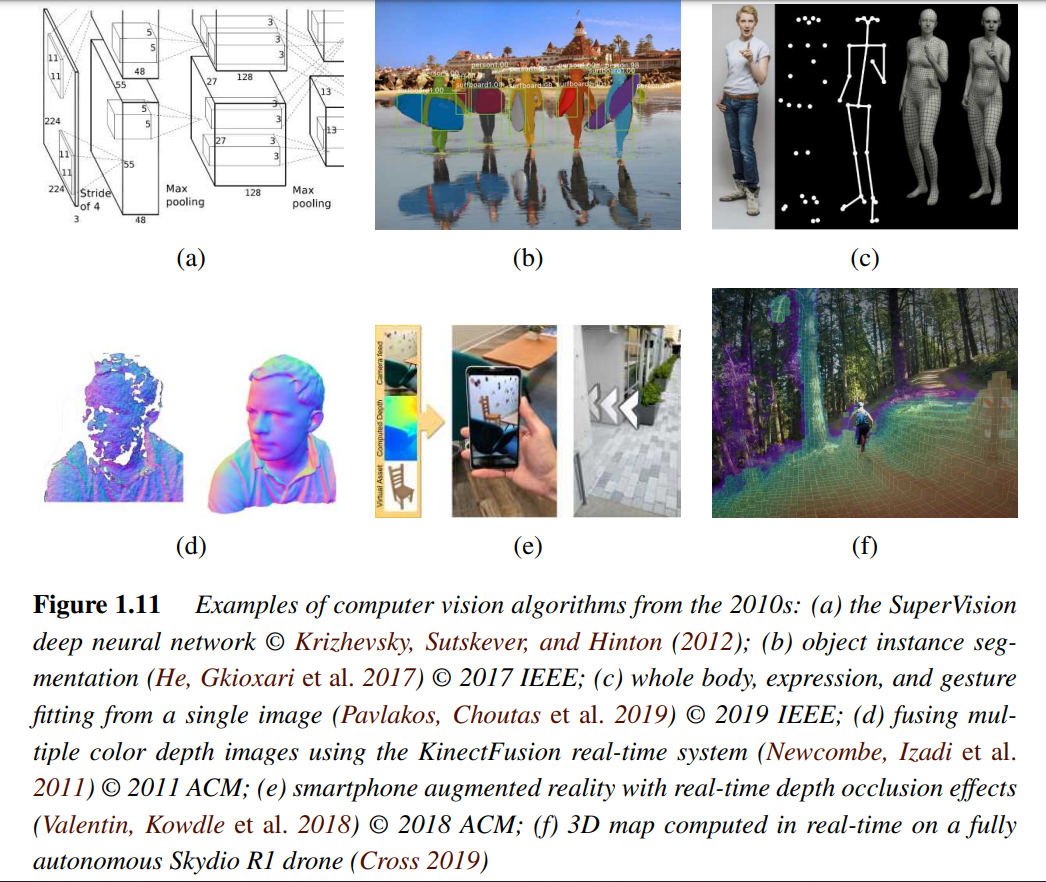
\includegraphics[width=0.75\textwidth]{img/10s.png}
\end{figure}

\subsection{Elementos}

Podríamos decir que los sistemas de visión por computador tienen en común:
Un sistema de captación y/o almacenamiento de imágenes, ya sea un físico (ej: cámara, escáner) o virtual (ej: recuperación de imágenes de internet).
Un sistema de preprocesamiento y adecuación de las imágenes para su uso.
La aplicación de técnicas para la extracción de información a partir de las imágenes. 
Realizar un proceso o tarea a partir de la información extraída, ya sea razonar o actuar (ej: vehículo autónomo), o generar una salida (ej: detección de objetos).

\subsection{Inspiración humana}

En términos generales el ojo y el cerebro humano son las fuentes principales de inspiración en la visión artificial, pero al haber aún mucho desconocimiento sobre el funcionamiento de este último siguen utilizándose técnicas matemáticas basadas en los pixeles de la imagen.

\vspace{\baselineskip}

Existe también inspiración humana en la funcionamiento de las CNN. El ojo humano detecta características geométricas de bajo nivel (líneas, bordes, esquinas) con las que agrupando jerárquicamente va identificando el objeto. Esto mismo se ha visto modelado en las capas de una CNN a diferentes profundidades. Además, estas características básicas son comunes entre objetos, y son las diferentes formas de combinarse las que los distinguen los unos de los otros.